% CREATED BY DAVID FRISK, 2015
\chapter{Discussion}

In the following chapter a discussion concerning the results and methods presented in the thesis is held. Apart from purely technical aspects...Finally some recommendations for further work is presented.

\section{Reflections}

\subsection{The connection of discrete and continuous models}
In this the method applies a discrete definition in continuous environment. The geodesic point definition is implemented on a continuous surface. This would not have been a problem if the surface would not have been generated from a discrete surface. I think the solution would have been more clean if the logic had been applied directly on the discrete surface. Clean or not it might the problem is the surface deviates more than what can be considered safe according to the rules of safety described in section.. If line of thrust is not further than 1/3 from the center it should be safe.

\subsection{ Polar geodesic coordinates}
In general the polar geodesics is a foundation as guidelines for the bricks. I think it is an easy method to understand as an designer, craftsman or an observer. It gives some sort of logic that is easy to understand and it feels harmonic. There are though some production and aesthetics issues that can arise. Firstly the closer one gets to the pole you might get issues since radius is decreasing but the bricks has the same size. Due to the brick size the bricks has a harder time adjusting to the small radius . The pole point itself will also need extra care and detailing. This is though an historic problem so there should be much research and examples of this already. One other issue is this discrete definition is that further away from the pole the bigger panels or coarser mesh. This means that the mesh is finer closer to the pole giving greater accuracy than further away. This might be a problem for structures that have shape that is somewhat rectangular in its vertical projection. Meaning that the surface needs to be divided into different areas with its own polar geodesic coordinates. One can see this phenomena in cathedrals with long aisles. 



\begin{figure}[H]
\centering
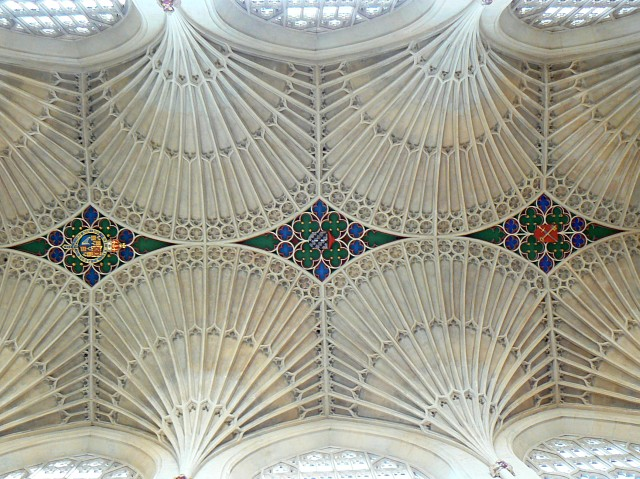
\includegraphics[width=1.0\linewidth ]{figure/Discussion/bathAbbey.jpg}
\caption{The fan vaults in Bath Abbey which has its own pole point in each fan vault.}
\end{figure}

\subsection{Discrete definitions}

The results from the test case proves that with a fine mesh this method can get results that are very close to a continuous version. The angle difference between the vectors was lower than 2 degrees and the median was 1.01 degrees. This proves that there is good probability that with a fine mesh one can simulate a analytical geodesic coordinate mesh on very complex surfaces. This means that it most likely be applied to form-found shapes of brick shells due to that they by their nature like to smooth to avoid tension.

\subsection{Parametric Environment} - This thesis did not aim to develop a fully functional parametric framework, but it intended the functionality to be part of it. One can ask if this parametric approach is somewhat is simplifying process, that it is more complex than be able to do thousand different options and more about understanding the context, the material, structural system etc. I do not think there is one program,script or parametric environment that can be applied to anything, since the meaning of parametric design is to define a solution space  For each project one must understand both the project and how this can be translated into a parametric scheme. To be able to do this one can have a tool box that helps you. This thesis addresses that the tessellation using polar geodesic coordinates could be one of these tools.

\subsection{Validity of the results}
It is hard to give a real number of within what domain the results get valid. The average results, on the shell, of both the geodesics points and the length between them should some significant good results. There were though some points that gave results that was not perfect. It is hard to say how big influence one point in a big mesh can have, what does one degree in that sense mean. It probably does not make much difference and the results of the test case proves that if one would have a much fines mesh it is not very interesting if one angle differs a bit for the geodesic, what is important is that the lengths of the geodesic segments are the same and that the angles of the mesh panels should be the same. Those are the properties of the analytical definition this method aims to achieve with a discrete solution.


\subsection{Computational efficiency}
The method of generating the geodesics, even though giving good results, needed much computer power and therefore took long time to produce. This limited how fine one would make the mesh of the geodesic coordinates. The discrete formulation is based on the fact that one simulate many points so that it resembles a continuous curve. This was hard to model due to the time it took to run a simulation. This also effected the possibility to do many different options and design. This area can be greatly improved and this thesis did not intend to find the most optimal way, but rather a way to produce geodesics and a geodesic coordinates mesh. In Rhinoceros3d there is for instance a command for creating a shortest path between two points. This is done very rapid so there is great potential in improving the computational power and speed required.     

\subsection{Edge conditions}

Considering build-ability one should think of how the edge conditions are related to the bed joints of the bricks. Choosing arbitrary edge boundaries can give make it necessary to make special bricks cut. This is not an optimal solution for a real project. Best thing would be to edge boundaries to follow the orthogonal trajectories so that they are level with the bed joints. Another solution would be to make for instance a concrete foundation that ends at an orthogonal trajectory so that the bricks starts in level with bed joints.

\begin{figure}[H]
\centering
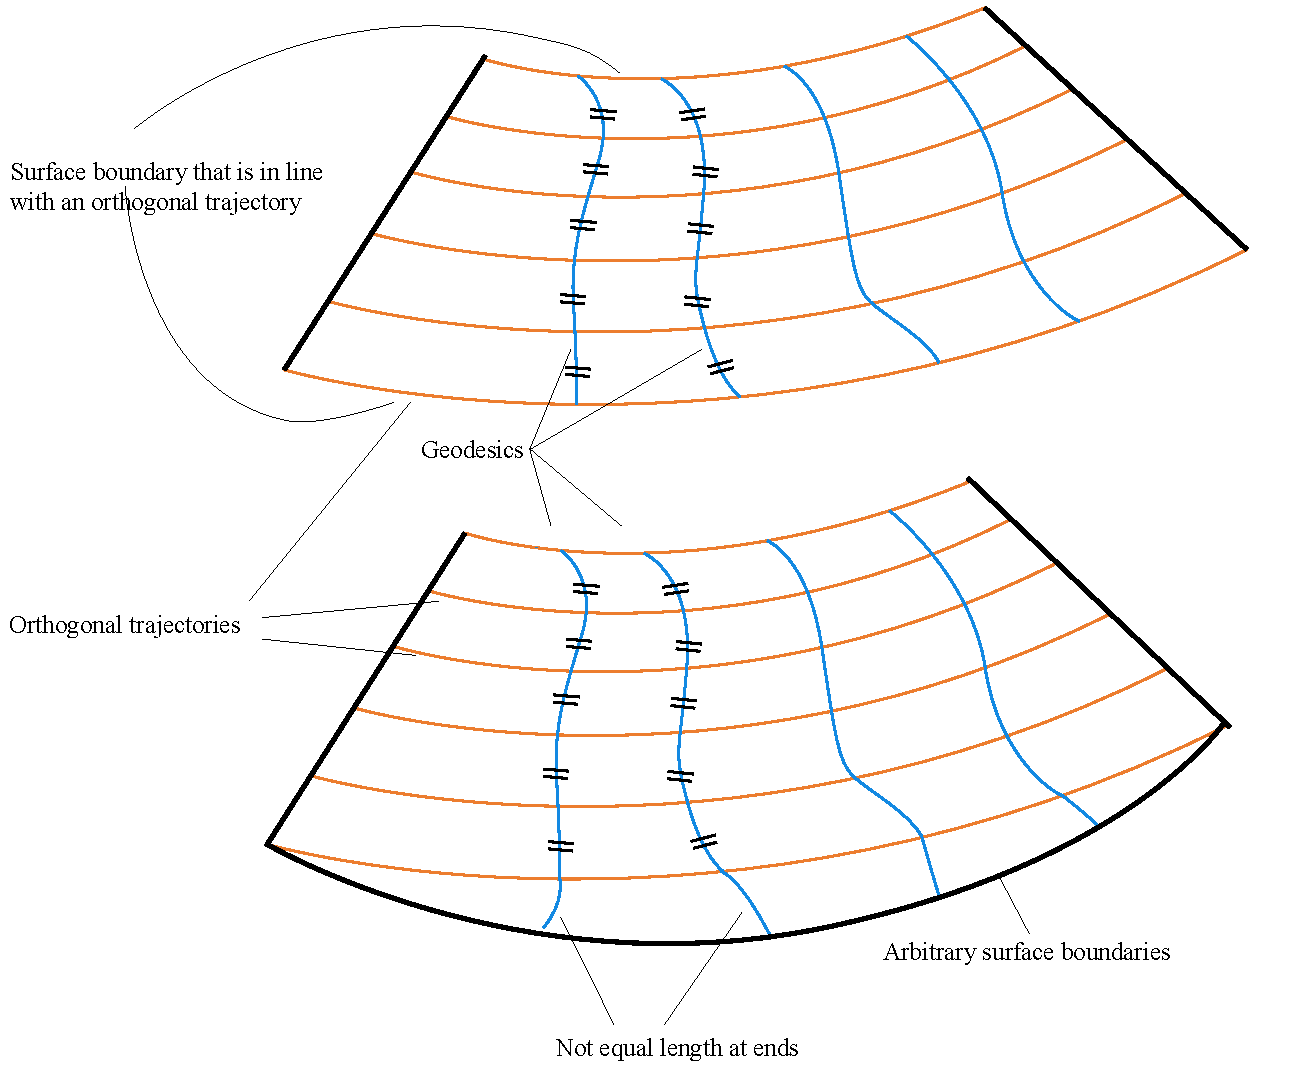
\includegraphics[width=1.0\linewidth ]{figure/Discussion/Boundaries.pdf}
\caption{The fan vaults in Bath Abbey which has its own pole point in each fan vault.}
\end{figure}

\section{Future work and improvements}

\begin{itemize}
    \item \textbf{Geodesic generation} - The speed of generating the geodesics using dynamic relaxation was successful but the method was computationally heavy. To solve this one could either find a more efficient method or solver for this matter. Since there already existed a dynamic solver this was not of priority to implement a new dynamic relaxation solver. Implementing a specialized solver can give many advantages. One could for instance set limits for which which the geodesic set is considered to be geodesic points, and focus its power on the sets that have harder time finding its position.
    
    \item \textbf{Implement general geodesic coordinates} - This thesis presents a method for generating general geodesic coordinates but whit-in the the time frame not possible to implement. General geodesic could be useful where the polar geodesic polar coordinates has disadvantages, as described in the reflections. 
    
    \item \textbf{Physical testing and validation} - To validate the results physical testing is usually the best method. In this thesis there was not time to make a real physical object challenging or proving the results. This could be good follow up in this subject to make both small models and a full scale mock-up that test this research question fully. Before a full scale model can be built a more rigorous structural design and assesment must be made.
    
   \item \textbf{Parametric Environment} - The work done in the parametric environment in Grasshopper3d   
   
    
\end{itemize}
